\title{Enhancing EDA and Misclassification Analysis through Tree Structure Visualization}
\author{
        Maor Hornstein \\
        \small{Tabular Data Science (89547) - Final Project}\\
}
\date{}

\documentclass[11pt]{article}
\renewcommand{\baselinestretch}{1.5}
\usepackage{graphicx}
\usepackage{caption}
\usepackage{refstyle}
\usepackage{xcolor}
\usepackage[labelsep=quad,indention=10pt]{subfig}
\usepackage[export]{adjustbox}
\usepackage{multirow}
\usepackage{array}
\newcolumntype{P}[1]{>{\centering\arraybackslash}p{#1}}
\usepackage{float}
\usepackage{algorithm}
\usepackage{algpseudocode}
\usepackage[round]{natbib} 

\newcounter{algsubstate}
\renewcommand{\thealgsubstate}{2.\arabic{algsubstate}}
\newenvironment{algsubstates}
  {\setcounter{algsubstate}{0}%
   \renewcommand{\State}{%
     \stepcounter{algsubstate}%
     \Statex {\footnotesize\thealgsubstate:}\space}}
  {}

\DeclareCaptionFont{gray}{\color{gray}}
\usepackage[font={color=gray}]{caption}

\renewcommand{\arraystretch}{1.5}

\begin{document}
\maketitle

\begin{abstract}
a short summary of the problem, your solution, and experimental results (up to 200 words).
\end{abstract}

\section{Problem Description}\label{Problem Description}
The focus of the solution is on the Exploratory Data Analysis (EDA) phase, particularly the use of scatter plots in this phase. \\
Scatter plots are a useful tool in data analysis and visualization due to their simplicity and ability to show the relationship between two or more groups. They are easy to comprehend and interpret, making them accessible for people with diverse backgrounds. Scatter plots help to uncover trends, patterns and outliers, examine the interactions between variables, and to highlight significant aspects of the data. \\
Despite their usefulness, scatter plots have some limitations. For instance, when data points are tightly packed or overlap (often referred to as overplotting), it can be challenging to accurately gauge the actual density of the data. Another significant challenge is distinguishing between groups when they overlap or when there is a small sample size. Lastly, Scatter plot only displays the distribution of the data in two dimensions and does not give insights into density or distribution in additional dimensions.

\section{Solution overview - The ICC plot}\label{Solution overview}
The proposed solution is a tree-based representation offered as an alternative to scatter plots to address their limitations.

The tree structure mimics the process a researcher goes through when analyzing a scatter plot, visually dividing the plane into subplanes and examining the density and distribution of samples in each subplane, as illustrated in \figref{fig1}.

\begin{figure}[H]
\centering
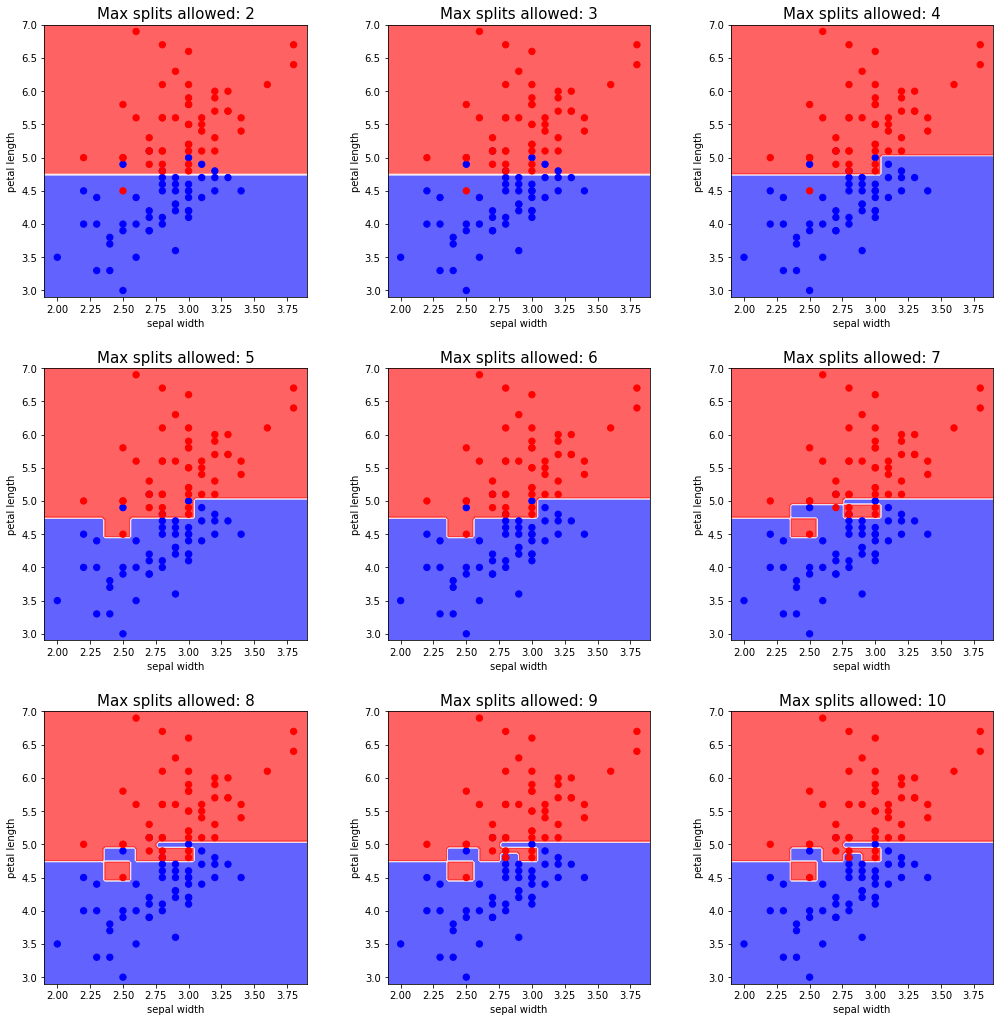
\includegraphics[width=0.8\textwidth]{scatter_plot_illustration.png}

\caption{Illustrates how a researcher visually divides the Scatter plot if he or she uses only horizontal and vertical lines. The simulation is based on a subset of the Iris dataset containing only the Versicolor and Virginica classes and the Sepal width and Petal length attributes.}
\label{fig:fig1}

\end{figure}

The selection of a tree structure representation was inspired by the widespread use of trees in daily decision making. Also, unlike the scatter plots that only feature points, a tree enables additional information to be displayed at its vertices and arcs. Last, the branching structure of the tree facilitates the analysis of multiple dimensions of the data. \\
Visual features such as colors and gradients aid in emphasizing the data's distribution, while confusion matrices at the tree nodes depict precisely the data's density. \\
I named the representation ICC plot, as an acronym of its 3 components: \textbf{I}nduction tree, \textbf{C}onfusion matrices and \textbf{C}olors.

\begin{figure}[H]
\centering
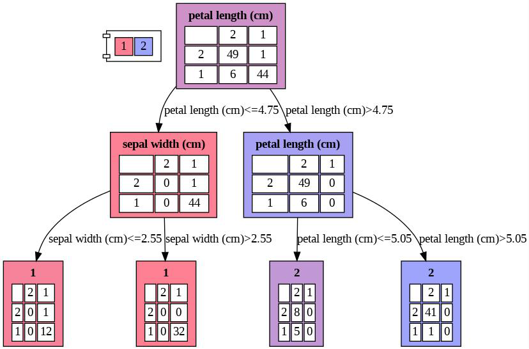
\includegraphics[width=0.8\textwidth]{icc.png}

\caption{ICC with 3 nodes simulate a plain with 3 splits.}
\label{fig:fig2}

\end{figure}

The ICC offers additional functionality to the researcher, such as adjusting the tree depth to increase or decrease the number of simulated splits of the plain, hiding the confusion matrices to focus on the data spread instead of specific quantities, and adjusting colors, as illustrated in  \figref{fig3}.

\begin{figure}[H]
        	\centering
           \subfloat{%
              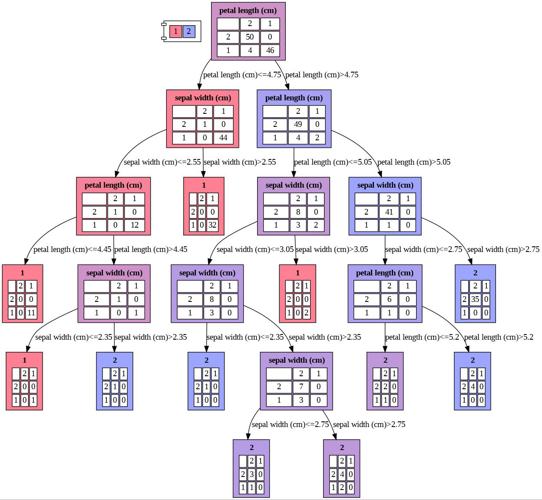
\includegraphics[height=3.5cm, valign=t]{ICC-v1.png}%
           } 
           \subfloat{%
              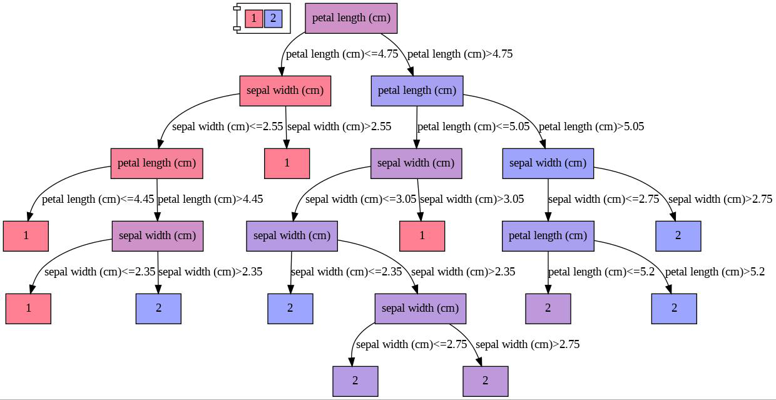
\includegraphics[height=2cm, valign=t]{ICC-v2.png}%
           }
           \subfloat{%
              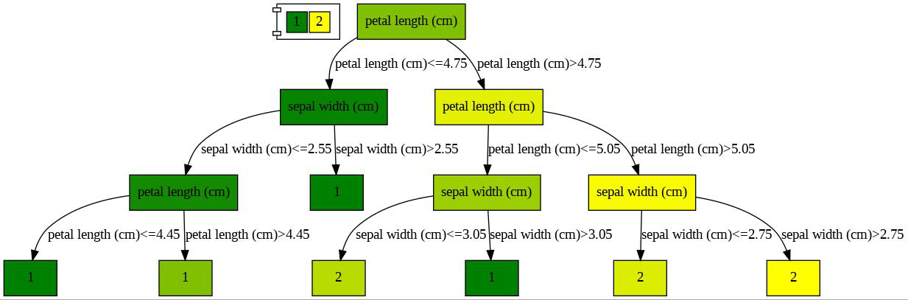
\includegraphics[height=2cm, valign=t]{ICC-v3.png}%
           }
           \caption{Different variations of ICC.}
           \label{fig:fig3}
\end{figure}    


\section{Experimental evaluation}\label{Experimental evaluation}
I evaluated the performance of the ICC plot by comparing it to Scatter and Jitter plots, as a baseline. To do this, I presented four CS students majoring in Data Science two graphs representing different datasets: one Scatter or Jitter plot, and the other - ICC plot. \\
In the first stage, I asked the students to write down as many observations as possible from each graph. In the second stage, I asked them to determine the relevance of their observations to the classification problem at hand. Finally, I asked them to share the advantages and disadvantages they came across during this evaluation for each graph type. \\
I repeated this process with three well-known datasets: Iris (to classify iris species), Titanic (to classify survivors and fatalities in the Titanic disaster), and Wisconsin breast cancer data\footnote{Only ten out of the thirty possible attributes in the Wisconsin breast cancer dataset were used in order to simplify the evaluation process.} (to classify a cell sample as malignant or benign). 

The results of the first two stages are presented in table \ref{table:tab1}.\\

\begin{table}[H]
\centering
\begin{tabular}{ |m{2cm}|m{4cm}||P{1.7cm}|P{1.7cm}|P{1.7cm}| } 
\hline
\multicolumn{2}{|m{3cm}||}{} & Iris data & Titanic data & Wisconsin breast cancer data \\
\hline
\hline
\multirow{2}{*}{\parbox{4cm}{Scatter\textbackslash\\Jitter plot}} & Mean number of observations according to the graph & 4.25 & 2 & 8.5 \\\cline{2-5}
& Percentage of observations relevant to the classification process &  27.9\% & 50\% & 23.6\% \\
\hline
\multirow{2}{*}{ICC} & Percentage of observations relevant to the classification process & 2 & 2 & 3.5 \\\cline{2-5}
& Percentage of observations relevant to the classification process &  79.1\% & 79.1\% & 75.4\% \\
\hline
\end{tabular}
\caption{Quantity and percentage relevance of insights provided by respondents for the classification problem discussed.}
\label{table:tab1}
\end{table}

The results show that scatter and Jitter plots are easier to draw insights from. On average, the scatter plots enabled to generate twice as many insights about the data compared to the ICC plot. However, the percentage of relevant insights for classification is low: for the ICC plot, almost 4/5 of the insights were relevant to the classification process compared to only one third for the Scatter and Jitter plots.\\
Based on the feedback from the subjects, it was revealed that the ICC graph was better suited for classification problems analysis but had two major drawbacks compared to the Scatter plot. Firstly, it was less intuitive and user-friendly and therefore required learning before using it. Secondly, the scatter plot made it easier to identify correlations, which was not possible in the ICC graph.

\section{Trying to take it one step forwards - The MAGIC tool}\label{Trying to take it one step forwards - The MAGIC tool}

As the ICC plot provides a convenient method to visualize data, it could potentially be utilized to analyze cases where a problem inherent in the data itself (rather than in the training process) results in misclassification of samples.\\
To test this, I propose algorithm \ref{alg:alg1}:\\
\begin{algorithm}
\caption{MAGIC algorithm}\label{alg:alg1}
\begin{algorithmic}[1]
	\State Build an ICC graph based on the training data.
	\State Trace the path of the test data on the ICC graph:
	\begin{algsubstates}
	\State Update the confusion matrices accordingly at each node.
	
	\State Mark nodes no test-data has passed through at all with white (These represent parts of the space that were present in the training data but are missing in the test data).
	\State Highlight nodes where samples of a different class than the one that appeared in the training set have reached with a double frame. 
\end{algsubstates}
\end{algorithmic}
\end{algorithm}

I developed an API that implements the algorithm mentioned above. The API not only generates the resulting tree but also enables extracting predicates representing a given test-sample according to it. I named the API the MAGIC (Misclassification Analysis by Graphic Induction-Tree Classifier) tool.\\
A sample of the MAGIC algorithm output is presented in \figref{fig:fig3}.

\begin{figure}[H]
\centering
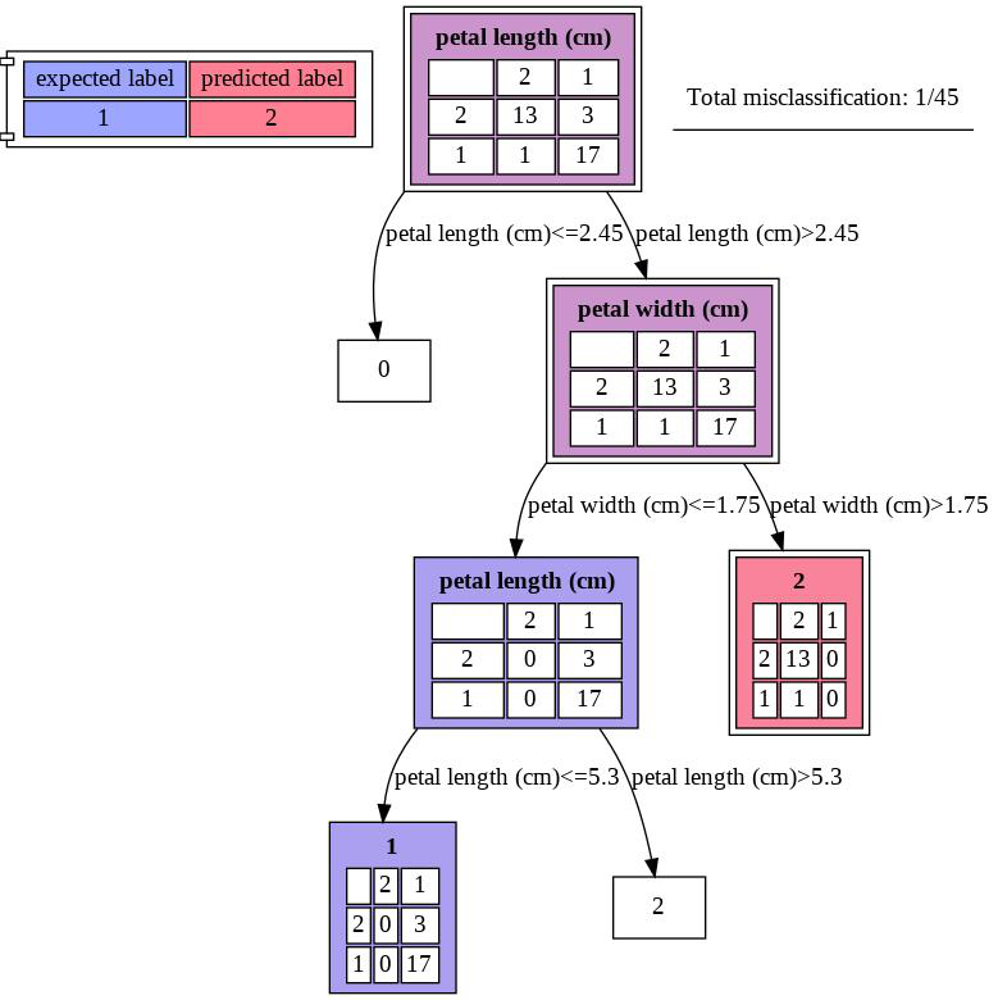
\includegraphics[width=0.8\textwidth]{iris-magic.png}

\caption{Examining test-data on a tree generated from the Iris dataset: The white vertices represent samples that are not present in the test data, for example, irises with a petal length of 2.45 or less. The double-framed vertices reveal that one sample in the test data was misclassified as a type 2 iris when it is actually a type 1. However, this error is understandable as 13 type 2 samples were correctly classified for similar reasons.}
\label{fig:fig3}

\end{figure}

\subsection{MAGIC Evaluation Process}\label{MAGIC Evaluation Process}
I conducted the evaluation process of the MAGIC tool in two stages.
The first stage involved a qualitative comparison of the MAGIC tool's performance with the Scatter plot on the three datasets used in the ICC evaluation. This comparison revealed that the MAGIC tool is particularly effective in identifying misclassification in two scenarios: (1) samples from different classes with overlapping characteristics and (2) samples from different classes with identical characteristics. Additionally, the tool proved useful in detecting Hidden Stratification, which I tested on a synthetically created dataset.\\
In the second stage of the evaluation, I used a rather humorous questionnaire for a quantitative measurement. Three out of the four subjects participated in the questionnaire, where they were presented with the data distribution of each of the four datasets using both tools, the MAGIC tool and the Scatter plot. The aim of the questionnaire was to determine the cases where they were able to successfully identify the reason for misclassification.

\subsection{MAGIC Evaluation Results}\label{MAGIC Evaluation Results}
From the qualitative research, it was found that the scatter plot graph is more effective in characterizing global phenomena, such as overlap in the characteristics of samples belonging to different classes, while the MAGIC tool is more useful for analyzing local cases, such as samples with identical or almost identical characteristics belonging to different classes, as mentioned above. Furthermore, the MAGIC tool was significantly useful for datasets where most of the characteristics were categorical because the Scatter Plot suffered from overplotting. The MAGIC tool was also found to be more useful in cases where misclassification was due to Hidden Stratification. The questionnaire results are presented on table \ref{table:tab2}.\\



\begin{table}[H]
\centering
\begin{tabular}{ |m{4cm}||m{4.5cm}|m{4.5cm}| } 
\hline
Reason for misclassificaion & Number of subjects who correctly identified the phenomenon using a Scatter plot & Number of subjects who correctly identified the phenomenon using the MAGIC tool \\
\hline
\hline
samples with identical characteristics & 1/3 & 2/3 \\
\hline
Samples with overlapping characteristics & 3/3 & 2/3 \\
\hline
Hidden Stratification & 1/3 & 2/3 \\
\hline
\end{tabular}
\caption{Quantity and percentage relevance of insights provided by respondents for the classification problem discussed.}
\label{table:tab2}
\end{table}

The subjects reported that the MAGIC tool was reasonably useful for the presented tasks, yet its main disadvantage is its visual complexity (due to the additional visual elements), which requires a significant learning curve. \\
As the MAGIC tool's strengths were found mainly in cases of local misclassification, it is better, then, to use more user-friendly tools, like LIME.


\section{Related work}\label{Related work}
\subsection{Scatter plots limitation}\label{Scatter plots limitation}
Although having quite a few limitations, Scatter plots have been widely used in the field of statistics and data analysis. Over time, researchers have proposed different improvements to overcome these limitations. I will briefly review a selection of works and solutions.\\
Scatter plots can get cluttered with large datasets and overlapping points, preventing the researcher from correctly assessing the density of the data. This is especially crucial when comparing between different groups. The oldest and most famous improvement for that is the Jittered Scatter plot, that randomly adjusts point positions to show data distribution better. \cite{woodruff1998constant} proposed a system named VIDA that plots dots for objects in dense regions and polygonal outlines for objects in sparser regions. \cite{dang2010stacking} suggested addressing the above by arranging points in a third dimension.\\
Another problem that the Overdraw poses is the difficulty of separating overlapping groups in the data. \cite{lee2012ieee} offer to use hierarchical multi-class sampling method to create a simplified, feature-preserving scatter plot visualization. \cite{mayorga2013splatterplots} propose to group dense data points and reveal subgroup relations through the use of smooth contour lines.\\
Oftentimes, two or three variables may not provide enough information to fully understand the relationships in the data. As plotting in four or more dimensions is impossible, Scatterplot Matrix (SPLOM) is commonly used. While solving the above, it imposes new challenges as it doesn’t scale with the features quantity[\citenum{carr1987scatterplot}][\citenum{lehmann2012selecting}].\\
Additional improvements might include employing Scagnostics methods[\citenum{sharma2012determining}], Spatial distortion[\citenum{keim1998gridfit}] and focusing on local patterns[\citenum{shao2016guiding}].

\subsection{Visualizing human decision making processes by trees
}\label{Visualizing human decision making processes by trees}

Trees are broadly used across different disciplines to analyze complex decision making processes and their outcomes. For example, the Ethno-graphic decision tree modeling[\citenum{gladwin1989ethnographic}] is a research method designed to identify the factors that groups of people use in their decision making. In game theory, the decision-making process is formalized and visualized using a tree, known as a \textit{game tree}[\citenum{gibbons1997introduction}].\\
Trees are available to professionals, such as psychological counselors, to aid in the counseling process[\citenum{beck2005ethnographic}] and for service providers to assess service provision[\citenum{harrison2018selecting}]. In political science, decision trees serve as a tool to analyze election results[\citenum{armengol2020decision}][\citenum{joynersimulating}].\\
The examples are many and varied. Ultimately, trees offer a graphical representation of intricate decision-making processes and assist in visually comprehending the connections between various factors and their effect on results.

\subsection{Misclassification Analysis}\label{Misclassification Analysis
}
Misclassification analysis is a crucial step in the Data Science pipeline, and as such, development environments designed for data scientists provide a variety of dedicated tools for it. For instance, Gestalt-20[\citenum{patel2010gestalt}] enables researchers to compare different samples side by side, making it possible to visually analyze differences between images in entity extraction tasks, or between texts in sentiment analysis tasks. ModelTracker[\citenum{amershi2015modeltracker}] is another tool that enables local examination of classification errors.\\
An example of a system in the text domain is EluciDebug[\citenum{kulesza2015principles}], which showcases the principle of Explanatory Debugging by reporting to the user why it classified a certain email in the way it did.\\
Finally, it is important to mention the well-known LIME algorithm[\citenum{ribeiro2016should}], which suggests using simpler and more interpretable models for misclassification analysis by examining the nearby and local environment of the misclassified sample.



\section{Conclusion}\label{Conclusion}
summarize your finding, and the things you learned from
the project

\setcitestyle{numbers}
\bibliographystyle{plainnat}
\bibliography{bib}

\end{document}